\chapter{Datenbank}\label{kap:Datenbank}
\section{Ziel der Datenbank}\label{kap:ZielDerDatenbank}
Die Datenbank soll möglichst den Aktuellen Zustand der Produktionsanlage Abbilden. Dazu gehören die Betriebsmittel wie zum Beispiel die Fertigungs-Stationen oder die Roboter mit ihren aktuellen Status und der Akkuleistung. Es sollen auch die Verwaltungsdaten wie Aufträge und Produktionsprozesse in der Datenbank gespeichert werden. Neben dem aktuellen Zustand der Produktionsanlage sollen auch die Fertigungsabläufe dort gespeichert werden. Dies beinhaltet in erster Linie eine Verfolgung der Werkstück durch Timestamps für das An- und Abmelden der Werkstück an den Bearbeitungsstationen. Es wird ebenso der Fortschritt den ein Werkstück im Fertigungsprozess und ein Auftrag insgesamt gemacht hat gespeichert. Eine weitere Aufgabe der Datenbank ist der Austausch von Daten zwischen dem Fertigungsrechner und der Fertigungsplanung. Alle Daten die zwischen diesen beiden Rechnern ausgetauscht werden, werden in die Datenbank geschrieben.
 
\section{Konzept} \label{kap:DatenbankKonzept}
Aus der realen Fertigungsanlage wird ein konzeptionelles Modell als Entität-Relationship-Diagramm modelliert. Das so modelliert ER-Diagramm ist in Abbildung \ref{fig:ER-Diagramm} zu sehen. Dazu werden insbesondere die Ziele aus Abschnitt \ref{kap:ZielDerDatenbank} berücksichtigt. Zur Qualitätssicherung wird sich an den drei gängigen Normalisierungsformen für Datenbanken orientiert. Anschließend wird das konzeptionelle Modell in ein logisches Datenschema überführt. Das Datenschema soll den ansprüchen eines relationalen Datenbankmodells entsprechen. 
\begin{figure}[h]
	    \centering
	    \includegraphics[width=1\linewidth]{Bilder/ERChanDiagramm.png}
        \caption{Entität-Relationship-Diagramm}
        \label{fig:ER-Diagramm}
\end{figure}
 
Zur Erstellung des konzeptionellen Modells wird für jede Betriebsmittelklasse der realen Anlage ein Entitätstyp angelegt. Es werden folgende Entitätstypen zur repräsentation von Bertiebsmitteln angelegt: Roboter, Arbeitsplatz, Parkplatz und Werkstück. Der Entitätstyp enthält die zu speichernden Attribute der Bertriebsmittel. So soll für das Betriebsmittel Roboter zum Beispiel die Attribute \glqq Akkuleistung\grqq  und \glqq Status\grqq  gespeichert werden. Neben den Entitätstypen für die realen Betriebsmittel werden auch Entitätstypen für die Daten, die zur Fertigungsplanung benötigt werden angelegt. Hierzu zählen die Entitätstypen: Auftrag und Produktionsprozess. Der Entitätstyp \glqq Timestamp\grqq  ist zur Speicherung der Fertigungsabläufe. Der Entitätstyp \glqq taggen\grqq  dient ausschließlich zur Kommunikation zwischen der Fertigungsplanung und dem Programm für die Ansteuerung der RFID-Schreib-/Leseköpfe. Zur Identifizierung der einzelnen Objekte enthält jeder Entitätstyp mindestens ein Antribut oder eine Kombination von Attributen, die die Entitäten eindeutig unterscheiden. Viele der Entitätstypen haben abgeleitet aus der realen Welt ein Attribut was die Entitäten unterscheidet. So ist zum Beispiel die Roboter ID ein Wert der sich aus der Nummerierung der Roboter in der realen Welt ableitet. Es gibt allerdings auch Entitätstypen die eigentlich kein einzelnes Attribut haben, dass sie eindeutig unterscheidet. Als Beispiel hierfür kann der Timestamp genannt werden, wo sowohl der \glqq Zeitstempel\grqq  als auch der \grqq Status\grqq  einen Entität nicht eindeutig identifizieren. Erst in Kombination mit der Beziehung zu einem Werkstück kann der Zeitstempel die Entitäten eindeutig unterscheiden. Zur einfacheren Handhabung des Timestamps wird dem Entitätstyp ein zusätzliches Attribut als \glqq id\_Timestamp\grqq  angelegt. Dabei handelt es sich um eine laufende Nummer die keinen zusätzlichen Informationen speichert sondern nur der einfacheren Verwaltung dient. Die Atribute oder kombinationen von Atributen die die Entitäten eines Entitätstyps eindeutig unterscheiden werden Schlüssel genannt. 
 
Da die Betriebsmittel der realen Welt ebenso wie die Daten der Fertigungsplanung oder die Feretigungsabläufe in Beziehung zu einander stehen werden die Entitätstypen mit Beziehungstypen verbunden und die jeweilige Beziehung deutlich gemacht. Es gibt je nach Art der Beziehung verschiedene Beziehungstypen zwischen den Entitätstypen. Es werden Beziehungstyp-Richtungen mit Kardinalität 1 oder Kardinalität N verwendet. Wobei die Beziehungstyp-Richtungen mit der Kardinalität 1 sowohl optional als auch nicht-optional vorkommen. Alle vorkommenden Beziehungstypen sind in Tabelle \ref{tab:Beziehungstypen} aufgeführt. Das bedeutet zum Beispiel für die Beziehung zwischen einem Timestamp und einem Werkstueck, dass ein Timestamp immer zu genau einem Werkstueck gehört, das Werkstueck aber kein, ein oder mehrere Timestamps haben kann. Es sich also um einen 1:CN Beziehungstyp handelt. Ein Parkplatz hingegen kann immer nur für einen oder keinen Roboter reserviert sein. Genauso kann ein Roboter immer nur an einem oder an keinem Parkplatz sein. Es handelt sich also um eine C:C Beziehung. 

\begin{table}[htbp]
    \centering	
    \captionof{table}{Beziehungstypen}
    \begin{tabular}{|p{4cm}|p{8cm}|} 
    \hline Beziehungstyp &  zwischen  \cr 
    \hline \hline  C:C &  taggen zu werkstueck\newline roboter zu parkplatz \newline roboter zu werkstueck \cr
    \hline C1:CN  & arbeitsplatz zu roboter \newline arbeitsplatz zu werkstueck \cr
    \hline 1:CN  & werkstueck zu timestamp \newline arbeitsplatz zu timestamp \newline auftrag zu werkstueck \newline produktionsprozess zu werkstueck \cr
    \hline 
    \end{tabular}
    \newline
    \label{tab:Beziehungstypen}
\end{table}

Beim entwerfen des Datenmodells mit einem Entitä-Relationship-Diagramm gillt es verschiedene Punkte zu beachten. Besonders wichtig ist es Redundanz bei Beziehungstypen und Atribute zu vermeiden. Bei Redundanz treten verschiedene Probleme auf. So müssen die selben Daten mehrfach in die Datenbank geschrieben werden und es wird außerdem unnötig Speicherplatz belegt. Diese Probleme sind aufgrund der relativ kleinen Datenbank und der geringen Anzahl an Usern nicht so relevant. Ein besonderes Problem könnte allerdings entstehen wen inkonsistente Daten entstehen weil nicht an allen Stellen die mehrfach vorhandenen Daten geändert wurden. Deshalb ist Redundanz zu vermeiden.
Ein gutes Beispiel für die Vermeidung von Redundanten Daten ist der Entitätstyp \glqq Produktionsprozess\grqq . Der Produktionsprozess hätte auch als Atribute direkt im Entitätstyp \glqq Werkstueck\grqq  gespeichert werden können, da aber jeder Produktionsprozess mehrfach vorkommt ist es sinnvoll diesen als eigene Objekt anzulegen und über eine Beziehung mit dem Werkstück zu verknüpfen. Sollte sich nun ein Produktionsprozess einmal ändern müsste nicht jedes Werkstück mit dem Produktionsprozess geändert werden sondern nur einmal die Objekt \grqq Produktionsprozess\grqq . Ebenso ist darauf zu achten keine redundanten Beziehungstypen zu modellieren. Eine Redundanz kann immer dann vermutetet werden, wenn zwei wege von einem Entitätstyp zu einem anderen Entitätstyp möglich sind.Beispielhaft sei hier der Entitätstyp \glqq Timestamp\grqq  genannt, der sowohl eine direkte Beziehung zum Entitätstyp \glqq Werkstueck\grqq  als auch eine indirekte Beziehung über den Entitätstyp \glqq Arbeitsplatz\grqq  hat. Da es sich bei den beiden Beziehungen des Timestamps allerdings um Zeitlich abgeschlossene Vorgänge handelt und die Beziehung zwischen Arbeitsplatz und Werkstück den aktuellen Zustand speichert kann von der Beziehung des Timestamps zum Arbeitsplatz nicht auf das dazugehörige Werkstück geschlossen werden, so dass die direkte Beziehung zum Werkstück notwendig ist.



\subsection{Normalisierung}
Anhand von Normalisierungsstuffen kann die Qualität eines Datenmodells beurteilt werden. Zur Qualitätssicherung wurden die ersten 3 Normalisierungsstuffen auf das in Abschnitt \ref{kap:DatenbankKonzept} beschriebene und in Abbildung \ref{fig:ER-Diagramm} dargestellte konzeptionelle Datenmodell. Durch die Anwendung der 3 Normalisierungsstuffen ensteht ein Datenmodell, dass in der 3. Normalform vorliegt. Das vorliegen in der 3. Normalform bitet auch bei der Überführung in das relationale Datenbank-Modell Vorteile bzw. ist bei Stuffe 1 sogar Voraussetzung.

\subsubsection*{1. Normalform}
Die erste Normalform besagt das eine Entität keine Attribute besitzen darf die zur gleichen Zeit mehrere Werte annehmen kann. So würde es zum Beispiel gegen die 1. Normalform verstoßen wenn die Zeitstempel als Attribut des Werkstücks angelegt worden währen, da dieses Attribut, je nach dem wie viele Stationen das Werkstück schon durchlaufen hat, mehrere Werte annehmen könnte. Um die 1. Normalform zu erreichen werden Attribute die mehrere Werte annehemn können aus dem Entitätstype herausgelöst und bilden einen Eigenen Entitätstype der durch einen Beziehungstype den Zusammenhang darstellt. Dabei hat die Beziehungstype-Richtung "Ursprüngliche Entitätstype zu neuem Entitätstype" die Kardinalität N oder CN.
Angewandt auf das Beispiel des Zeitstempels wurde, wie in Abbildung \ref{fig:ER-Diagramm} zu sehen ist, der Zeitstempel in den neuen Entitätstype Timestamp ausgelagert. Der Beziehungstype-Richtung von Werkstück zu Timestamp ist CN.
Ein Wert welcher nicht aus einer Liste besteht oder anders aus mehreren Werten zusammengesetzt ist wir als atomarer Wert bezeichnet. Für ein relationales Datenbank-Modell gilt: Jeder Wert eines Attributes muss ein atomarer Wert sein.\cite{Jarosch:2016}

\subsubsection*{2. Normalform}
Damit ein Datenmodell in der 2. Normalform vorliegt muss es sich in der ersten Normalform befinden. Zusätzlich darf jedes Attribut ausschließlich vom Gesamtschlüssel eines Entitätstyps funktional Abhängig sein. Funktional Abhängigkeit bedeutet, dass aus dem Wert von Attribut A sich automatisch der Wert von Attribut B ergibt. Zum verdeutlichen der zweiten Normalform nutze ich ein etwas konstruiertes Beispiel. Angenommen die Produktionsanlage fährt mit zwei verschiedenen Typen von Robotern. Mit jeweils zwei alten Festo-Robotern und zwei neuen von studenten Entwickelten Robotern. Die id der Roboter setzt sich nun aus zwei Ziffern zusammen die jeweils ein E
eigenes Attribut bilden und zusammen den Gesamtschlüssel für den Entitätstyp Roboter. Die erste Ziffer währe dabei entweder eine 1 für die Festo-Roboter oder eine zwei für die neuen Roboter. Die zweite Ziffer ist eine laufende Nummer. Wird jetzt zusätzlich das Baujahr gespeichert und sind die Roboter eines Typs jeweils im gleichen Jahr gebaut so liegt eine funktionale Abhängigkeit zwischen dem Attribut Baujahr und dem Teilschlüssel erste Ziffer vor. Um die zweite Normalform nun herzustellen wird der Teilschlüssel und das abhängige Attribut herausgelöst und Sie bilden einen neuen Entitätstyp. Die zweite Normalform verringert Redundanzen innerhalb des Datenmodells.\cite{Heuer:2001}

\subsubsection*{3. Normalform}
Damit ein Datenmodell in der 3. Normalform vorliegt muss es sich in der 2. Normalform befinden und zusätzlich darf eine Attribut eines Entitätstyps nicht transitiv funktional abhängig sein.  So wäre es zum Beispiel möglich die Attribute des Entitätstyps Produktionsprozesses mit im Entitätstyps Werkstück zu speichern. Es läge dann allerdings eine transitive funktionale Abhängigkeit zwischen den Werten der Attribute Station 1 bis 5 und Dauer Station 1 bis 5 und dem Schlüssel RFID Werkstück vor, da die AttributeStation 1 bis 5 und Dauer Station 1 bis 5 funktional von der id\_Produktionsprozess abhängig währen. Die id\_Produktionsprozess wiederum wäre wiederum funktional abhängig vom Schlüssel RFID Werkstück. Deshalb wird dieser Teil herausgelöst und bildet einen eigenen Entitätstyp. Die dritte Normalform verringert die gefahr von Redundanzen im Datenmodell.\cite{Heuer:2001}

\section{relationales Datenbankmodell}\label{kap:relationales_Datenbankmodell}
Bei einer MySQL-Datenbank handelt es sich um eine relationale Datenbank. Dabei entspricht eine Entität aus dem ER-Diagramm einem Tupel von Werten und der Entitätstyp einem Relationstyp. 

So lässt sich nun die Mengen aller Entitäten eines Entitätstyps als Tabelle darstellen. Dabei entsprechen die Überschriften der einzelnen Spalten den Namen der Attribute. Eine Zeile repräsentiert dann jeweils eine Entität bzw. ein Tupel von Werten. Wie schon beim ER-Diagramm hat jeder Relationstyp ein oder mehrere Attribute die als Primärschlüssel dienen. Beziehungstypen werden über sogenannte Fremdschlüssel realisiert. Fremdschlüssel stellen eine zusätzliche Spalte in einer Tabelle da. Ist in einer Tabelle ein Fremdschlüssel eingetragen referenziert dieser auf eine  Zeile einer anderen Tabelle und stellt so die Beziehung her. Dabei muss stets die referenzielle Integrität dieser Verweise gewährleistet sein, dass bedeutet das ein Fremdschlüssel immer auf eine Vorhandene Zeile einer anderen Tabelle referenziern muss oder mit einen NULL-Marker belegt sein muss. 

\section{Zugriff auf die Datenbank}\label{kap:DatenbankZugriff}
Die MySQL-Datenbank ist auf einem Server, der auf dem Fertigungsrechner läuft, implementiert. Es gibt zwei User die Zugriff auf die Datenbank benötigen. Das ist zum einen die Fertigungsüberwachung, die das auslesen der RFID-Chips übernimmt und die Fertigungsplanung. Die Fertigungsüberwachung befindet sich auf dem selben Rechner wie der Server der Datenbank. Die Fertigungsplanung ist auf einem anderen Rechner realisiert und über Ethernet mit dem Fertigungsrechner verbunden. Die Fertigungsplanung ist mit Qt ausgeführt und hat über eine eingebundene Bibliothek über Ethernet direkten Zugriff auf die Datenbank. Die Fertigungsüberwachung läuft auf einer Soft-SPS auf dem Fertigungsrechner und ist mit CoDeSys programmiert. Ein direkter Zugriff von der Soft-SPS auf die Datenbank ist nicht möglich. Ein Zugriff könnte über einen OPC-Server erfolgen. OPC (Open Platform Communications) ist ein standartisierte Softwareschnitstelle. Sie ermöglicht den Datenaustausch zwischen Steuerungen verschiedenen Herstellern aus der Automatisierungstechnik. Hier wurde allerdings ein anderes Verfahren, speziell für den Zugriff auf Datenbanken von Steuerungen aus der Automatisierungstechnik, angewandt. Es handelt sich dabei um den SQL4Automation Connector der Firma Inasoft Systems GmbH. Der SQL4Automation connector ist speziell für den Zugriff von Speicherprogramierbaren Steuerungen auf eine Datenbank entwickelt und ermöglicht sowohl Lese- als auch Schreibbefehle in SQL direkt auf der SPS zu Programmieren. Für die verwendete Steuerung ist schon eine fertige Bibliothek vorhanden, was die Anwendung deutlich erleichtert. In Abbildung \ref{fig:DatenbankZugriffUebersicht} ist Schematisch dargestellt wie auf die Datenbank zugegriffen wird.

\begin{figure}[ht]
	    \centering
	    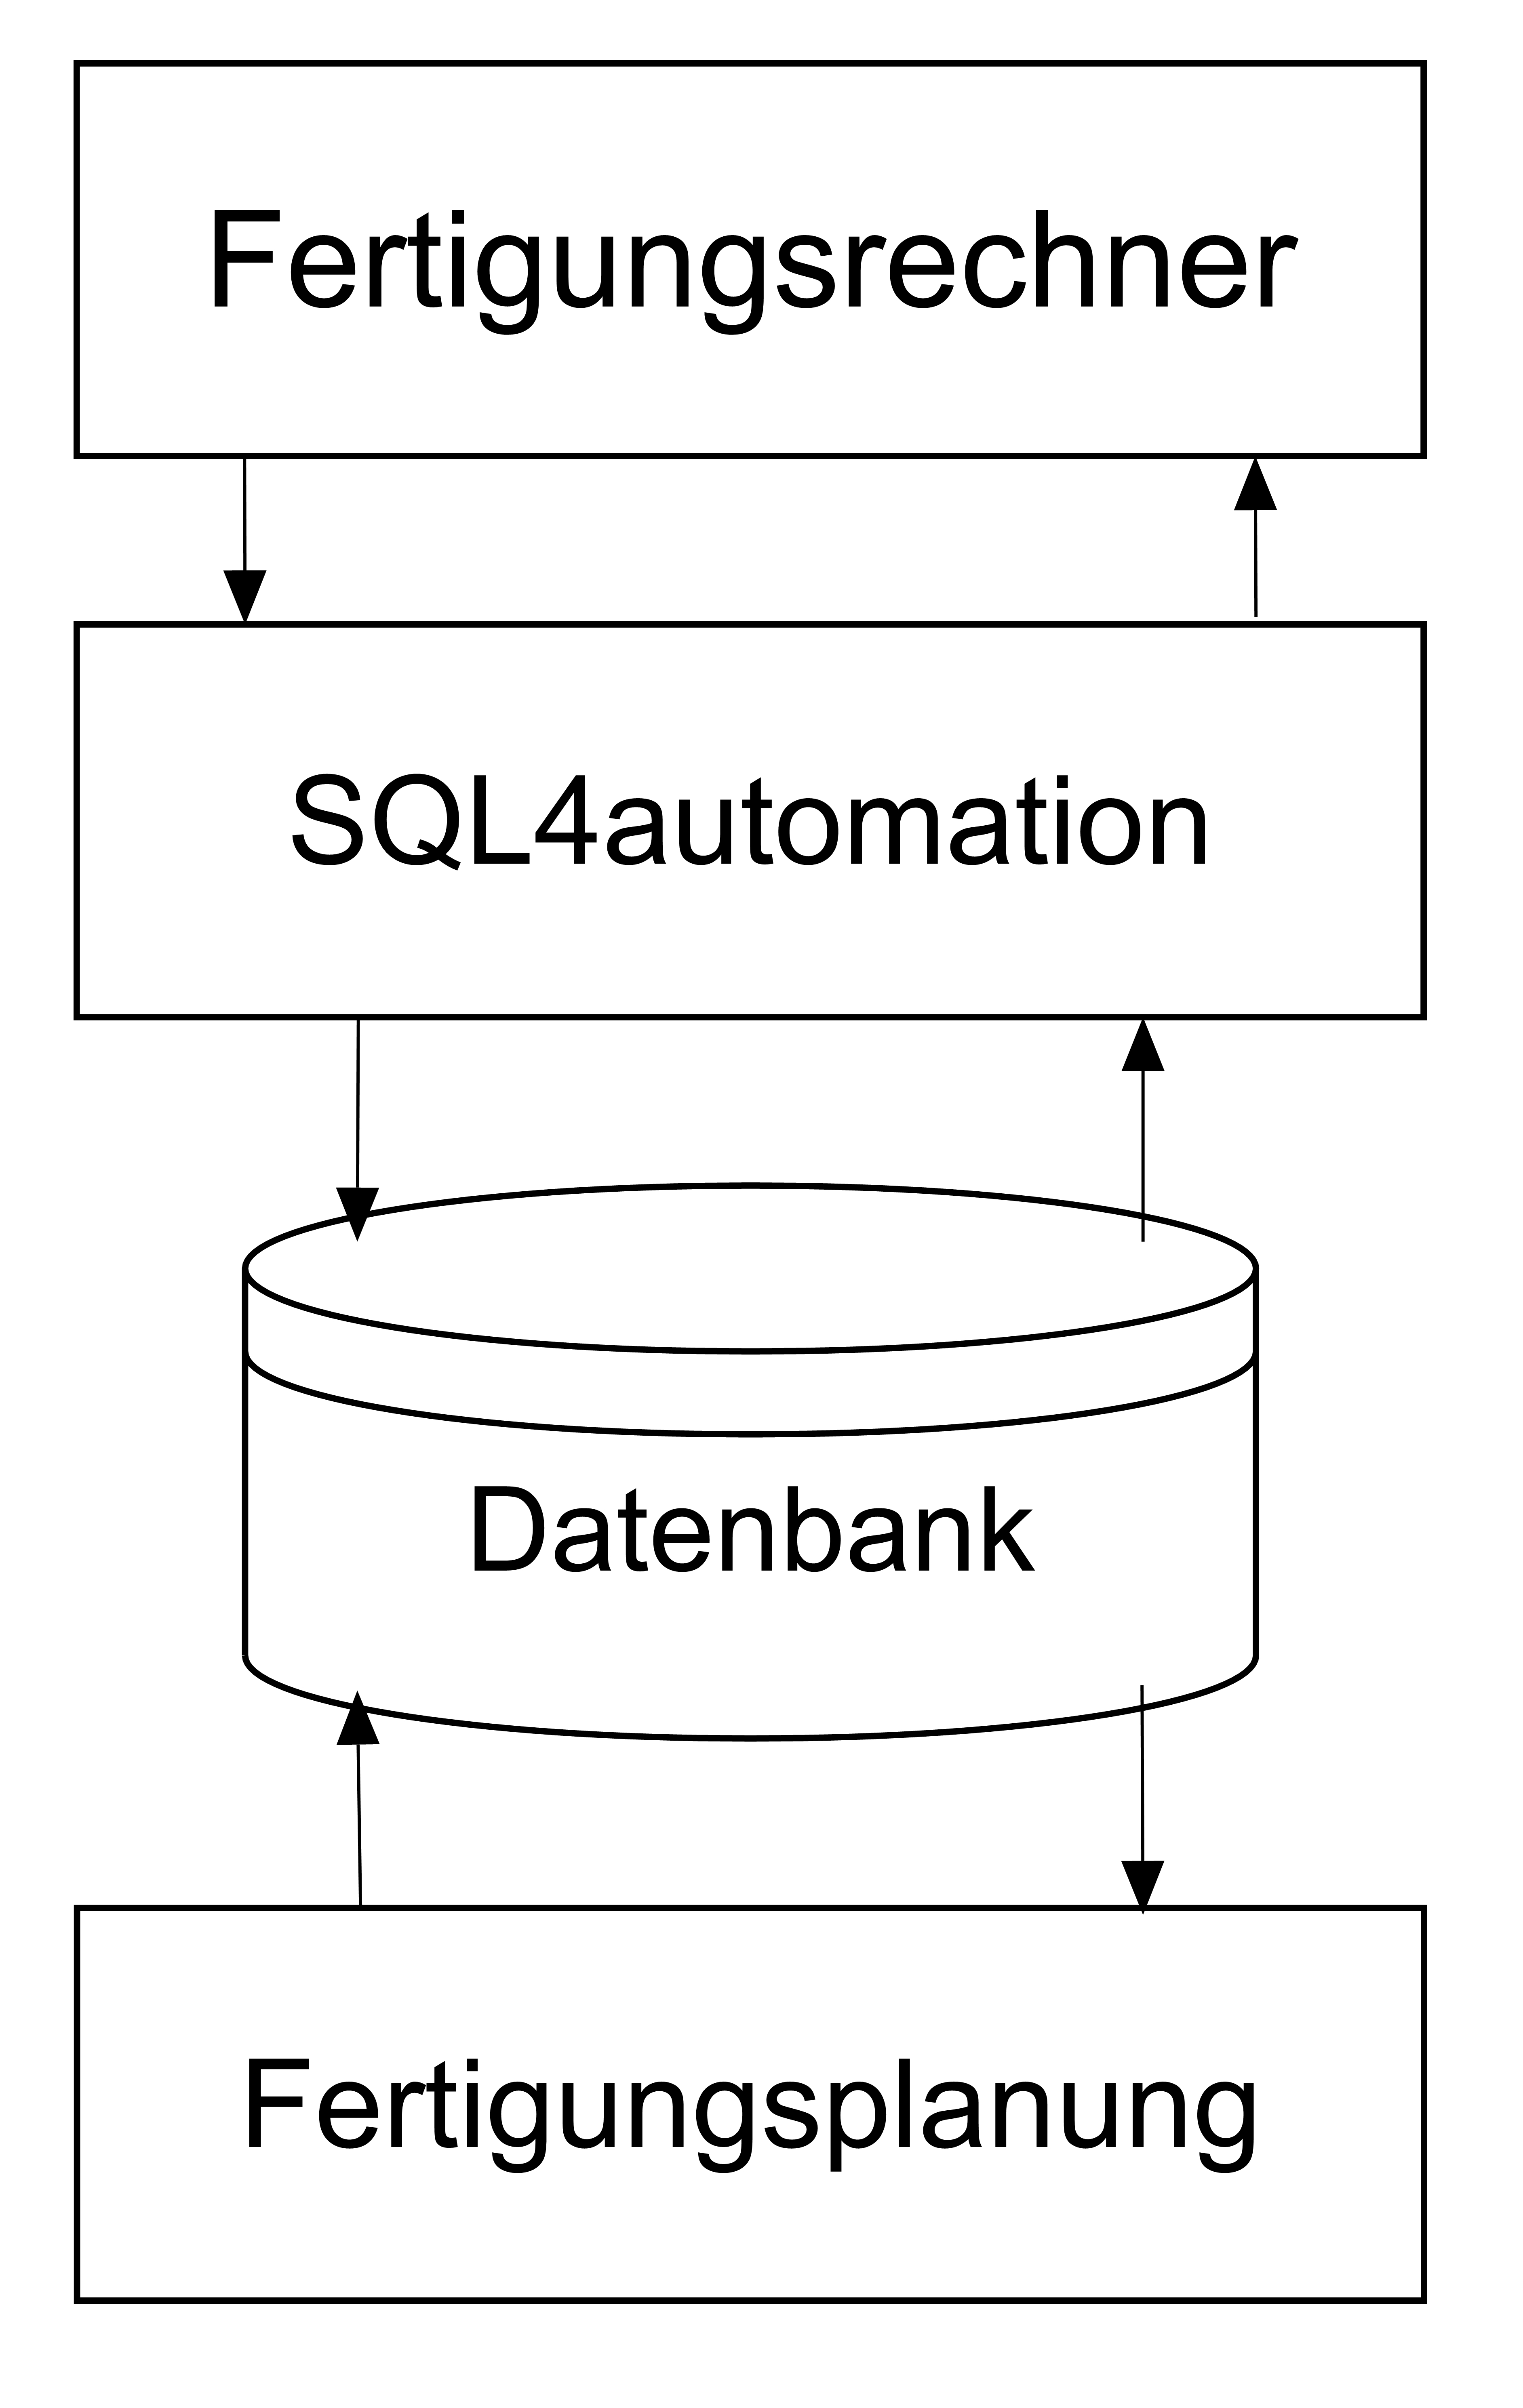
\includegraphics[width=0.4\linewidth]{Bilder/Datenbankdiagramm.png}
        \caption{Schematische Darstellung des Datenbankzugriffs}
        \label{fig:DatenbankZugriffUebersicht}
\end{figure}


\section{Vorgehen}
 Zunächst wurde anhand des in Abschnitt \ref{kap:DatenbankKonzept} beschriebenen Konzeptes das ER-Diagramm der Datenbank graphisch Entwickelt. Das so entstandene ER-Diagramm ist in Abbildung \ref{fig:ER-Diagramm} zu sehen. Die Entwicklung des ER-Diagramms erfolgte in enger Absprache mit der Fertigungsplanung, da diese einer der Hauptuser der Datenbank ist.
 
\begin{figure}[ht]
	    \centering
	    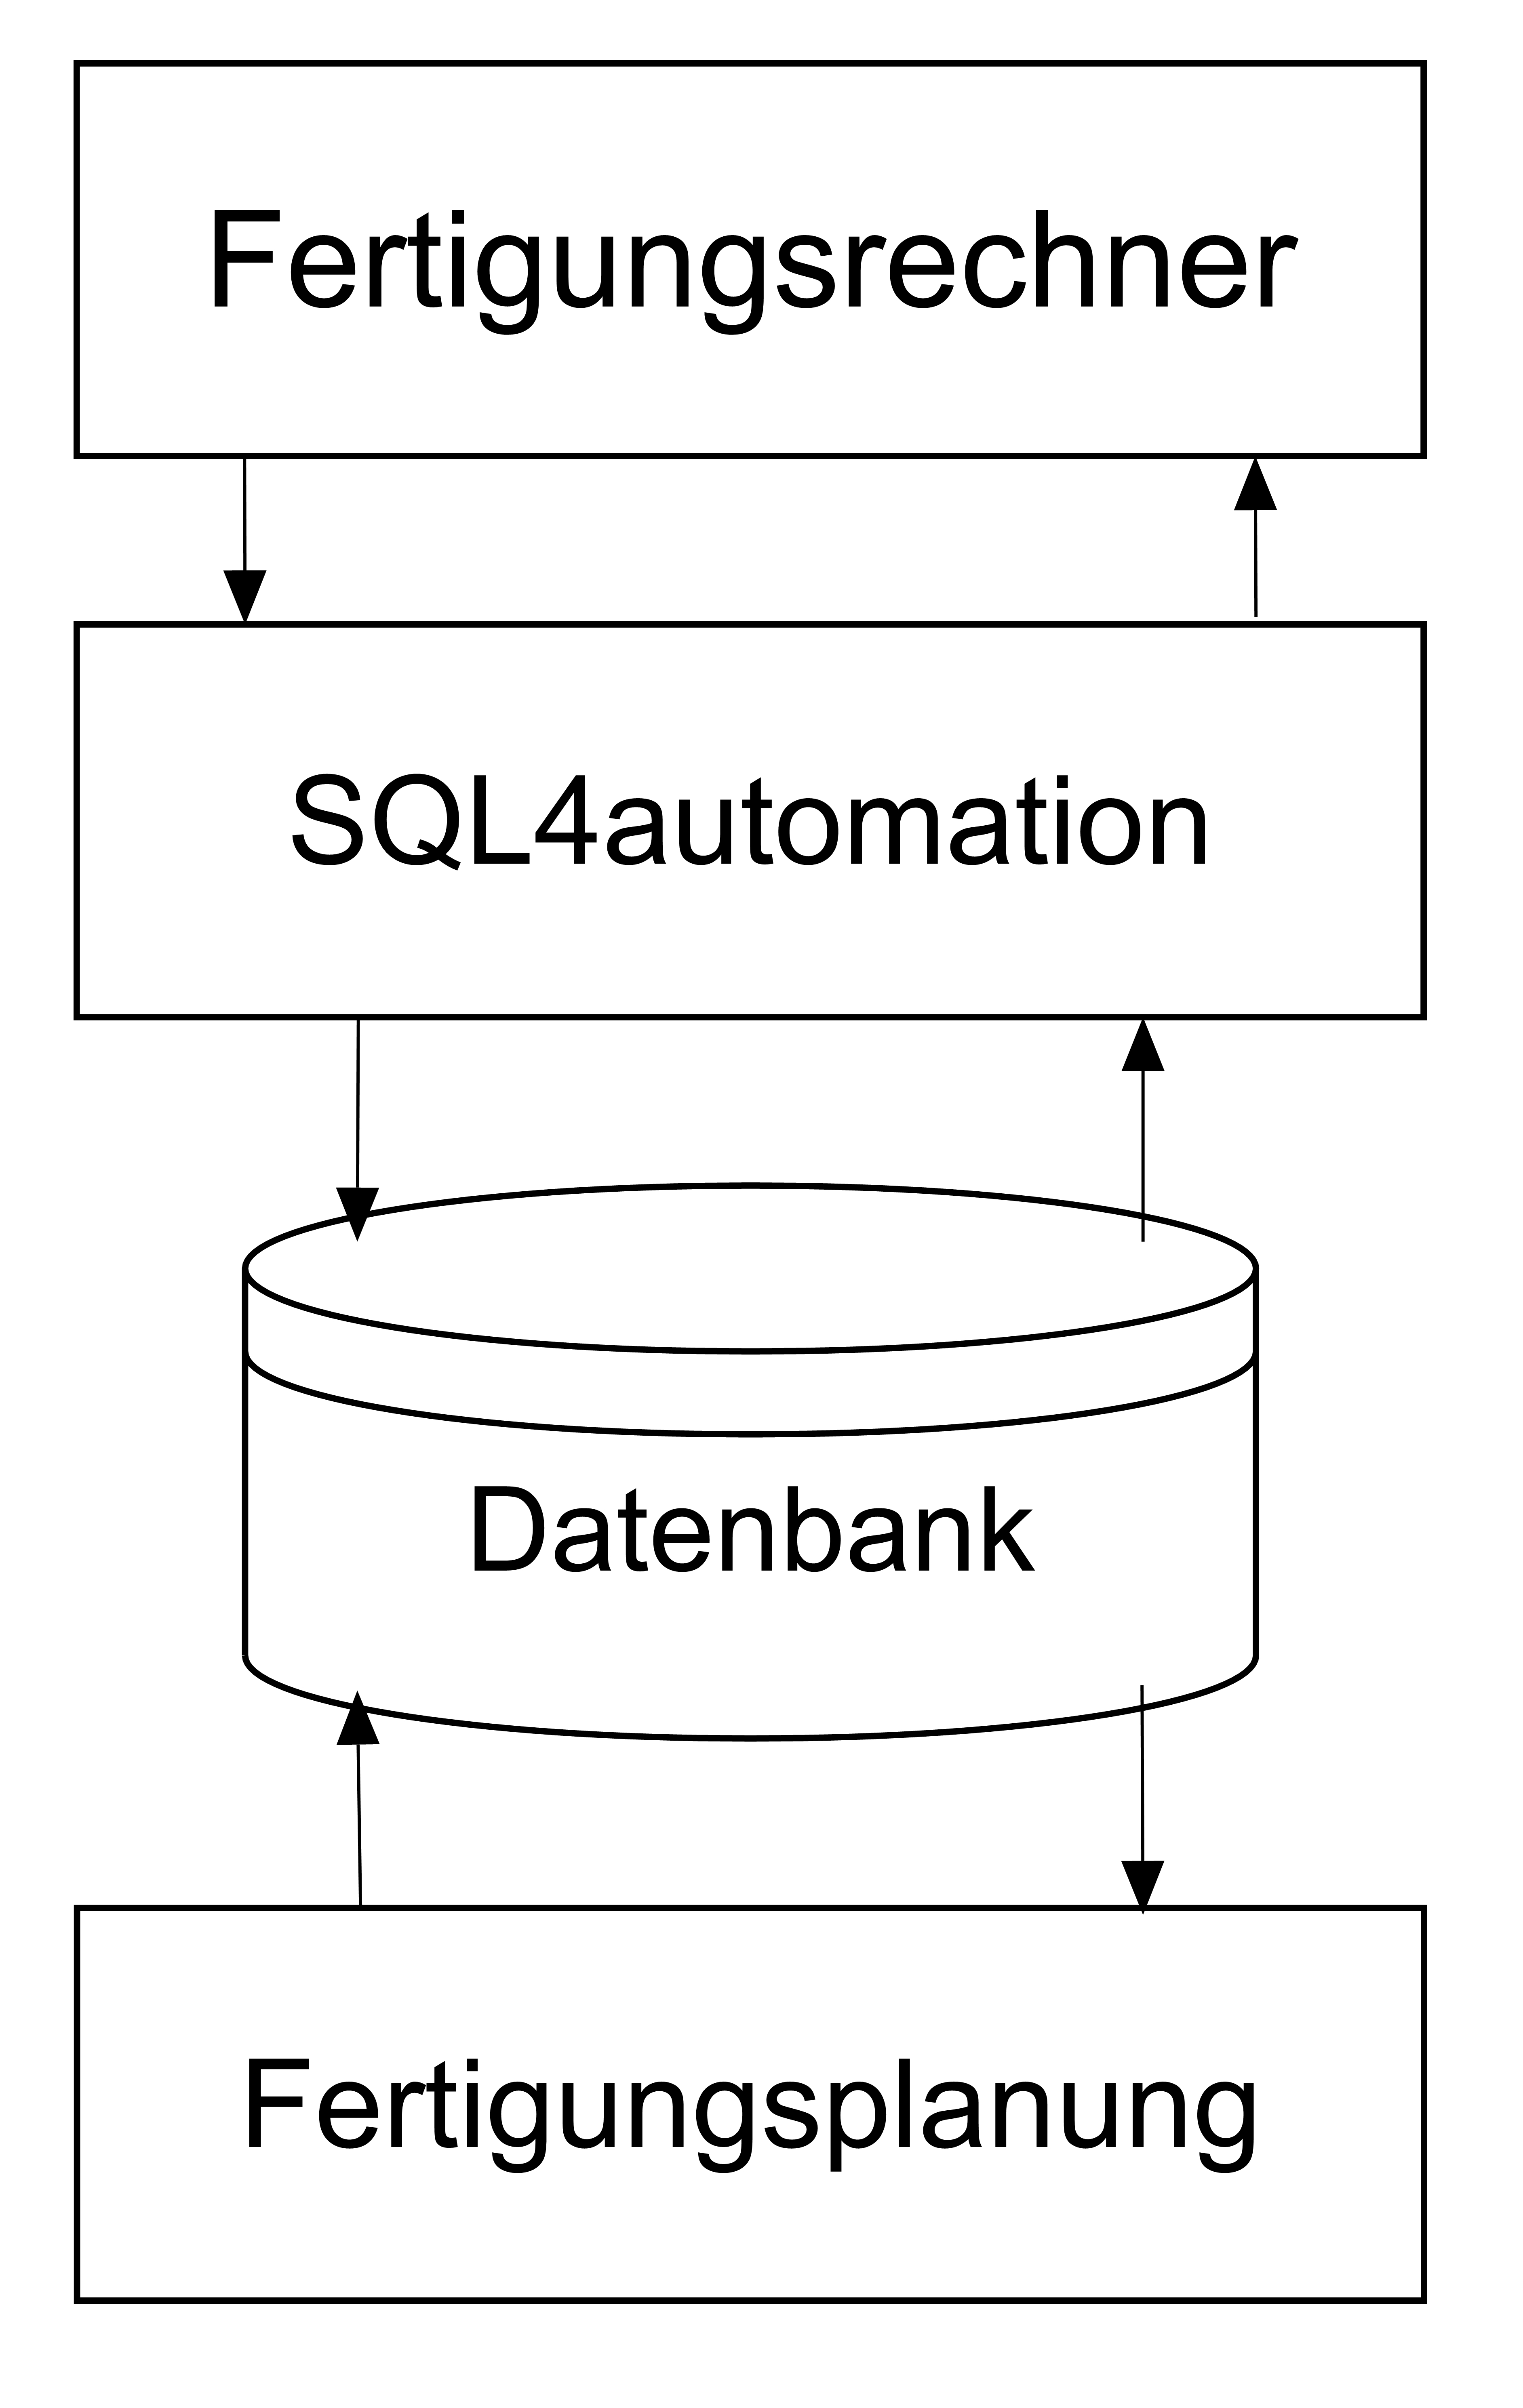
\includegraphics[width=0.4\linewidth]{Bilder/Datenbankdiagramm.png}
        \caption{Grafisches-Modell der Datenbank}
        \label{fig:ER-Diagramm_Worbenche}
\end{figure}
 
 Zum erstellen der Datenbank wurde das Tool MySQL-Workbenche vom Entwickler Oracle Corporation genutzt. Dieses Tool ermöglicht die visuelle Entwicklung, Erstellung und Bearbeitung einer Datenbank. És können außerdem MySQL-Befehle zum Beispiel zum Testen ausgeführt werden. Die visuelle Entwicklung erfolgt über die graphische Eingabe des aus dem ER-Diagramm entwickelten relationalen Datenbankmodells wie in Abbildung \ref{fig:ER-Diagramm_Worbenche}. In der Tabelle \ref{tab:ER-Erklaerung} sind die Symbole die durch die MySQL-Workbenche verwendet werden beschrieben.
%\begin{comment}
\begin{table}[ht]%{1\textwidth}
    \centering	
    \captionof{table}{Beziehungstypen}
    \begin{tabular}{|H{1cm}|p{8cm}|} 
    \hline Zeichen &  Bedeutung  \cr 
    \hline \hline   
\includegraphics[width=0.5cm,]{Bilder/ER/Primaerschluessel.PNG} &  Primärschlüssel \cr
    \hline 
\includegraphics[width=0.5cm,]{Bilder/ER/EigenschaftNN.PNG}  & Eigenschaft (darf nicht NULL sein) \cr
    \hline 
\includegraphics[width=0.5cm,]{Bilder/ER/Eigenschaft.PNG}  & Eigenschaft \cr
    \hline 
\includegraphics[width=0.5cm,]{Bilder/ER/FremdschluesselNN.PNG}  &  Fremdschlüssel (darf nicht NULL sein)\cr
    \hline 
\includegraphics[width=0.5cm,]{Bilder/ER/Fremdschluessel.PNG}  & Fremdschlüssel \cr
    \hline 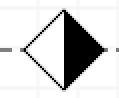
\includegraphics[width=0.5cm,]{Bilder/ER/1zuN.PNG}  & 1:N Beziehung \cr 
    \hline 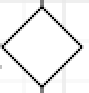
\includegraphics[width=0.5cm,]{Bilder/ER/1zu1.PNG} &  1:1 Beziehung \cr
    \hline 
    \end{tabular}
    \newline
    \label{tab:ER-Erklaerung}
\end{table}
%\end{comment}
 Es können dort die Entitätstypen welche in das relationale Datenbankmodell transformiert einer Tabelle entsprechen angelegt werden. Jeder Tabelle kann ein Primärschlüssel und Eigenschaften zugewiesen werden. Sowohl dem Primärschlüssel als auch den Eigenschaften müssen ein Datentyp zugewiesen werden. Es können auch weitere Festlegungen für die Eigenschaften getroffen werden. So kann eine Eigenschaft als \glqq NOT NULL\grqq  festgelegt werden, was bedeutet das beim Anlegen einer neuen Entität Beziehungsweise einer neuen Zeile in der Tabelle diese Eigenschaft immer gesetzt werden muss und auch nicht später gelöscht werden kann. So muss zum Beispiel ein Parkplatz immer einen Status haben. Beim Produktionsprozess, der nicht immer die selbe Länge hat, ist es nicht notwendig das alle Eigenschaften immer einen Wert haben. So brauch ein Produktionsprozess mit nur 4 Stationen die Eigenschaften \glqq station\_5\grqq  und \glqq dauer\_station\_5\grqq  nicht. Der Primärschlüssel muss selbstverständlich immer vergeben werden und darf nicht mit einem  NULL-Marker belegt sein.
 Auch Beziehungstypen können in der MySQL-Workbenche selbstverständlich abgebildet werden. Wird ein Beziehungstyp angelegt, so erzeugt dieser automatisch den, wie in Abschnitt \ref{kap:relationales_Datenbankmodell} beschrieben, dazugehörigen Fremdschlüssel in den jeweiligen Tabellen. Je nach Beziehungstyp dürfen diese durch einen NULL-Marker belegt  sein oder müssen eine Wert haben. So kann bei einer optionalen C1:CN Beziehung, wie sie zum Beispiel von Arbeitsplatz zu Roboter besteht, das Feld für den Fremdschlüssel auch \glqq NULL\grqq  sein. Bei einer 1:CN Beziehung wie vom Auftrag zum Werkstueck darf der Fremdschlüssel \glqq auftrag\_id\_auftrag\grqq  beim Werkstück nicht mit einem NULL-Marker belegt sein, da jedes Werkstück einem Auftrag zugeordnet werden muss.
 
 Nach dem grafischen Entwurf der Datenbank kann mittels der Option \glqq Forward Engineer to Database\grqq  aus dem grafischen Modell automatisch der entsprechende Code für die Datenbank erstellt werden und die Datenbank ohne weitere Programmierung erstellt werden. Auch nachträgliche Änderungen oder Erweiterungen an der Datenbank können direkt im grafischen Modell erfolgen und über die \glqq Forward Engineer to Database\grqq  Option direkt eingepflegt werden. So bleibt das grafische Modell und die Datenbank immer auf dem selben Stand. Es ist keine zusätzliche pflege der Dokumentation während des Entwicklungsprozess nötig. 
 
 Nach dem erstellen der Datenbank lässt sich die Struktur der Datenbank im Navigator der MySQL-Workbenche betrachten. Zum Befüllen der Datenbank lassen sich über das Abfrage-Fenster MySQL-Befehle wie zum Beispiel \glqq INSERT INTO\grqq  ausführen. Beim Befüllen ist insbesondere darauf zu achten die Tabellen in der richtigen Reihenfolge zu befüllen. So kann ein Werkstück zum Beispiel erst angelegt werden wenn der dazugehörige Auftrag bereits erstellt wurde.
 
 Über das Abfrage-Fenster lassen sich auch die MySQL-Befehle die später im CoDeSys-Programm auf der Soft-SPS so wie im mit Qt entwickelten Programm auf dem Fertigungsrechner implementiert werden testen. Es hat sich für die Implementierung in Qt herausgestellt das es sinvoll ist zunächst mit einem SET-Befehl eine Variable zu deklarieren und ihr einen Wert zuzuweisen. Das erhöht die Lesbarkeit des Codes, da die eigentliche Abfrage nicht zerschnitten werden muss. Im Listing \ref{lst:MySQLQt} ist Beispielhaft der Code für die Abfrage ob und welcher Arbeitsplatz an einer Station frei ist dargestellt. Die Zuweisung zur Variable \glqq @Station1\grqq  ist dabei nur Beispielhaft und erfolgt eigentlich über eine Variable in Qt. Diese Abfrage liefert eine 1 zurück sollten beide (Zeile 4) oder der erste (Zeile 5) Arbeitsplatz der entsprechenden Station frei sein. Ist nur der zweite Arbeitsplatz frei liefert die Abfrage eine 2 (Zeile 6) und sollten alle Arbeitsplätze belegt sein  wird eine 0 zurückgeliefert (Zeile 7).
 
\lstset{ 
    keywordstyle        =\bfseries\ttfamily\color{blue},
    basicstyle          =\scriptsize\ttfamily, 
    emphstyle           =\color{red},
    numbers             =left,
    xleftmargin         =15pt,
    backgroundcolor     =\color{lightgray},
    showstringspaces    =false,
    language            =SQL
    }	 

\begin{lstlisting}[caption={MySQL-Befehl: Freier Arbeitsplatz }
       \label{lst:MySQLQt},
       captionpos=t] 
SET @Station1 = 40; 
SELECT
    (CASE
        WHEN(SUM(id_Arbeitsplatz))=@Station1+1+@Station1+2 THEN 1 
        WHEN(SUM(id_Arbeitsplatz))=@Station1+1 THEN 1 
        WHEN(SUM(id_Arbeitsplatz))=@Station1+2 THEN 2 
        ELSE 0 
    END) 
FROM 
    vpj.arbeitsplatz 
WHERE (id_Arbeitsplatz IN (@Station1+1,@Station1+2) 
        AND Werkstueck_RFID_Werkstueck is NULL);
\end{lstlisting}

Bei den MySQL-Abfragen handelt es sich meistens um Abfragen die nur einen Wert zurück liefern und keine ganzen Tabellen, so dass die Rückgabewerte direkt eine Aussage treffen und nicht die  Tabellen erneut durchsucht werden müssen. Ziel war es die Abfragen so präzise wie möglich zu gestalten um die Nachbearbeitung der Abfrage-Ergebnisse weitestgehend zu verhindern. Eine Ausnahme stellen hierbei die Daten da die später als Listen in der Visualisierung ausgegeben werden. Beispielhaft seien hier die RFID-Timestamps mit den dazugehörigen Zeiten und Arbeitsplätzen genannt die als Liste zurückgegeben werden.

Das erstellen der MySQL-Befehle lief nach und nach parallel zur Entwicklung der beiden User-Programme der Datenbank. Zunächst wurde die Anforderung an den Befehl festgelegt. Anschließend wurde der Befehl erstellt und mit der MySQL-Workbenche getestet. Nach dem Erfogreichem Test wurde der Befehl in seine Zielumgebung, also CoDeSys oder Qt, portiert und dort erneut getestet. Beim Testen der Befehle ist insbesondere der Error Code interessant. Der Error Code liefert wichtige Hinweise weshalb ein Befehl nicht funktioniert. Der Error Code kann anhand von Error Code Listen dekodiert werden. Für die Tests in der MySQL-Workbenche übernimmt das dekodieren die Entwicklungsumgebung.